\documentclass[a4paper,12pt,english]{article}
\usepackage{glossaries}
\usepackage[T1]{fontenc}
\usepackage{babel}
\usepackage{graphicx}
\usepackage[table,xcdraw]{xcolor}
\usepackage{hyperref}
\usepackage{blindtext}
\usepackage{geometry}
\usepackage{parskip}
\usepackage{mathtools}
\usepackage{siunitx}
\usepackage{listings}
\usepackage{csquotes}
\usepackage{caption}
\usepackage{subcaption}
\usepackage{comment}
\usepackage{pdfpages}
\usepackage[useregional]{datetime2}
\usepackage{amsmath} % for the equation* environment
\usepackage{float}
\usepackage{pict2e}
\usepackage{fixltx2e}
\usepackage{tocloft}
\usepackage{graphicx}
\usepackage{xcolor}
\usepackage{float}
\usepackage{textgreek}
\usepackage{colortbl}
\usepackage{multirow}


%%gmedina solution
\newcommand{\listequationsname}{List of equations}
\newlistof{myequations}{equ}{\listequationsname}
\newcommand{\myequations}[1]{%
\addcontentsline{equ}{myequations}{\protect\numberline{\theequation}#1}\par}
\setlength{\cftmyequationsnumwidth}{2.5em}% Width of equation number in List of Equations

\DeclareRobustCommand{\slashcirc}{{\mathpalette\doslashcirc\relax}}

\makeatletter
\newcommand\doslashcirc[2]{%
  \sbox\z@{$#1\m@th\circ$}%
  \setlength\unitlength{\wd\z@}
  \begin{picture}(1,1)
  \roundcap
  \put(0,0){\box\z@}
  \put(0,0){\line(1,1){1}}
  \end{picture}%
}
\makeatother



\definecolor{stmblue}{RGB}{0,114,198}    % Adjusted STM32 blue color
\definecolor{stmgray}{RGB}{128,128,128}
\definecolor{stmgreen}{RGB}{34,177,76}    % Adjusted STM32 green color
\definecolor{stmorange}{RGB}{255,140,0}
\definecolor{codegreen}{rgb}{0,0.6,0}
\definecolor{codegray}{rgb}{0.5,0.5,0.5}
\definecolor{codepurple}{rgb}{0.58,0,0.82}

\lstset{
  language=C,
  basicstyle=\ttfamily\footnotesize,
  keywordstyle=\color{stmblue},
  stringstyle=\color{stmgreen},
  commentstyle=\color{stmgray},
  moredelim=[s][\color{stmorange}]{\#}{\ },
  frame=tb,
  tabsize=4,
  showstringspaces=false,
  breaklines=true,
  numbers=left,
  numberstyle=\tiny\color{stmgray},
  numbersep=5pt,
  extendedchars=true,
  keywords=[2]{HAL_TIM_OC_Start,HAL_TIM_PWM_Start,HAL_TIM_Base_Start_IT,HAL_ADC_Start,HAL_ADC_PollForConversion,HAL_I2C_Init,Error_Handler,HAL_SPI_Init,CDC_Transmit_FS,HAL_TIM_PWM_Init,HAL_TIMEx_MasterConfigSynchronization,HAL_TIM_PWM_ConfigChannel,HAL_TIM_MspPostInit,    HAL_ADC_Init,HAL_ADC_Start,HAL_ADC_Stop,HAL_ADC_PollForConversion,HAL_ADC_GetValue,HAL_ADC_MspInit,HAL_ADC_MspDeInit,HAL_CAN_Init,HAL_CAN_ConfigFilter,HAL_CAN_Start,HAL_CAN_Transmit,HAL_CAN_Receive,HAL_CAN_MspInit,HAL_CAN_MspDeInit,HAL_CRC_Init,HAL_CRC_Accumulate,HAL_CRC_Calculate,HAL_CRC_MspInit,HAL_CRC_MspDeInit,HAL_DAC_Init,HAL_DAC_Start,HAL_DAC_Stop,HAL_DAC_SetValue,HAL_DAC_MspInit,HAL_DAC_MspDeInit,HAL_DCMI_Init,HAL_DCMI_Start,HAL_DCMI_Stop,HAL_DCMI_MspInit,HAL_DCMI_MspDeInit,HAL_DMA_Init,HAL_DMA_DeInit,HAL_DMA_Start,HAL_DMA_Start_IT,HAL_DMA_Abort,HAL_DMA_PollForTransfer,HAL_DMA_GetState,HAL_DMA_IRQHandler,HAL_ETH_Init,HAL_ETH_DeInit,HAL_ETH_Start,HAL_ETH_Stop,HAL_ETH_Transmit,HAL_ETH_Transmit_IT,HAL_ETH_TransmitFrameReadyCallback,HAL_ETH_Receive,HAL_ETH_Receive_IT,HAL_ETH_IRQHandler,HAL_ETH_MspInit,HAL_ETH_MspDeInit,HAL_FLASHEx_DATAEEPROM_Unlock,HAL_FLASHEx_DATAEEPROM_Lock,HAL_FLASHEx_DATAEEPROM_Erase,HAL_FLASHEx_DATAEEPROM_Program,HAL_FLASHEx_DATAEEPROM_EnableFixedTimeProgram,HAL_FLASHEx_DATAEEPROM_DisableFixedTimeProgram,HAL_FLASHEx_DATAEEPROM_LaunchFixedTimeProgram,HAL_FLASHEx_DATAEEPROM_GetStatus,HAL_FLASHEx_DATAEEPROM_IRQHandler,HAL_FLASHEx_DATAEEPROM_Callback,HAL_FLASHEx_DATAEEPROM_IT_IRQHandler,HAL_FLASHEx_DATAEEPROM_IT_Callback,HAL_GPIO_Init,HAL_GPIO_DeInit,HAL_GPIO_WritePin,HAL_GPIO_ReadPin,HAL_GPIO_TogglePin,HAL_GetTick,HAL_GetTickFreq,HAL_GetTickPrio,HAL_GetHalVersion,HAL_GetREVID,HAL_GetDEVID,HAL_GetUID,HAL_Init,HAL_DeInit,HAL_MspInit,HAL_MspDeInit,HAL_PCD_Init,HAL_PCD_DeInit,HAL_PCD_SetupStageCallback,HAL_PCD_ResetCallback,HAL_PCD_SuspendCallback,HAL_PCD_ResumeCallback,HAL_PCD_SOFCallback,HAL_PCD_ISOOUTIncompleteCallback,HAL_PCD_ISOINIncompleteCallback,HAL_PCD_DataOutStageCallback,HAL_PCD_DataInStageCallback,HAL_PCD_ConnectCallback,HAL_PCD_DisconnectCallback,HAL_PCD_MspInit,HAL_PCD_MspDeInit,HAL_PCDEx_PMAConfig,HAL_PCDEx_LPM_Callback,HAL_PCDEx_BCD_Callback,HAL_RCC_OscConfig,HAL_RCC_ClockConfig,HAL_RCCEx_PeriphCLKConfig,HAL_RCC_GetOscConfig,HAL_RCC_GetClockConfig,HAL_RCC_GetPeriphCLKConfig,HAL_RCC_OscConfigPLL,HAL_RCC_ClockConfig_PLL,HAL_RCC_OscConfigSaiPLL,HAL_RCCEx_EnableLSE,HAL_RCCEx_DisableLSE,HAL_RCCEx_EnableMSIPLLMode,HAL_RCCEx_DisableMSIPLLMode,HAL_RCCEx_EnablePLLSAI1,HAL_RCCEx_DisablePLLSAI1,HAL_RCCEx_EnablePLLSAI2,HAL_RCCEx_DisablePLLSAI2,HAL_RCCEx_GetPeriphCLKConfig,HAL_RCCEx_PeriphCLKConfig,HAL_RCCEx_ClockSecuritySystem_Enable,HAL_RCCEx_ClockSecuritySystem_Disable,HAL_RCCEx_WakeUpStopCLKConfig,HAL_RCCEx_EnableSRAM2Clock,HAL_RCCEx_DisableSRAM2Clock,HAL_RCCEx_EnableFMCMemorySwapping,HAL_RCCEx_DisableFMCMemorySwapping,HAL_RTC_Init,HAL_RTC_DeInit,HAL_RTC_MspInit,HAL_RTC_MspDeInit,HAL_RTCEx_BKUPWrite,HAL_RTCEx_BKUPRead,HAL_RTCEx_SetTime,HAL_RTCEx_SetDate,HAL_RTCEx_SetAlarm,HAL_RTCEx_SetTimeStamp,HAL_RTCEx_DeactivateTimeStamp,HAL_RTCEx_SetWakeUpTimer,HAL_RTCEx_SetCoarseCalib,HAL_RTCEx_DeactivateCoarseCalib,HAL_RTCEx_EnableBypassShadow,HAL_RTCEx_DisableBypassShadow,HAL_RTCEx_GetTime,HAL_RTCEx_GetDate,HAL_RTCEx_GetAlarm,HAL_RTCEx_GetTimeStamp,HAL_RTCEx_GetWakeUpTimer,HAL_RTCEx_GetCoarseCalib,HAL_RTCEx_GetSynchroShift,HAL_RTCEx_GetTimeStamp_IT,HAL_RTCEx_GetWakeUpTimer_IT,HAL_RTCEx_PollForTimeStamp,HAL_RTCEx_PollForWakeUpTimerEvent,HAL_RTCEx_WakeUpTimerIRQHandler,HAL_RTCEx_Tamper1EventCallback,HAL_RTCEx_Tamper2EventCallback,HAL_RTCEx_TimeStampEventCallback,HAL_RTCEx_AlarmAEventCallback,HAL_RTCEx_AlarmBEvent,TIM2_IRQHandler},
    keywordstyle=[2]{\color{stmblue}},
keywords=[3]{htim1,htim2,htim3,htim4,htim5,htim6,htim7,htim8,htim9,htim10,i,hadc1,hadc2,hadc3,j,TIM_CHANNEL_1,TIM_CHANNEL_2,TIM_CHANNEL_3},
    keywordstyle=[3]{\color{stmorange}}
}




\usepackage[
    backend=biber,
    backref=true,
    backrefstyle=none,
    sortcites=true,
    sorting=none,
    doi=false, % doi informatie wordt niet weergegeven
    %uniquename=true,
    %uniquelist=true,
    maxcitenames=3,
    %issn=false, werkt niet
    language=american
]{biblatex}
\addbibresource{information/Sources.bib}
\DefineBibliographyStrings{english}{
    backrefpage = {page},
    backrefpages = {page},
}
\makeglossaries
\definecolor{Grey1}{HTML}{343434}
\graphicspath{{./img}}
 \geometry{
 a4paper,
 total={170mm,257mm},
 left=20mm,
 top=20mm,
 }
\hypersetup{
    colorlinks=true,
    linkcolor=blue,
    filecolor=magenta,      
    urlcolor=cyan,
    pdftitle={Overleaf Example},
    pdfpagemode=FullScreen,
    }


\begin{document}

\include{main/front}
\maketitle

\include{information/VersionHistory}
\include{information/Glossary}
\include{information/ListOfFigures}
\include{main/TableOfContents}

%% Use Arabic numerals for the page numbers of the chapters.
%\mainmatter %% fix dit MARNIX

\section{Components}
\begin{figure}[H]
    \centering
    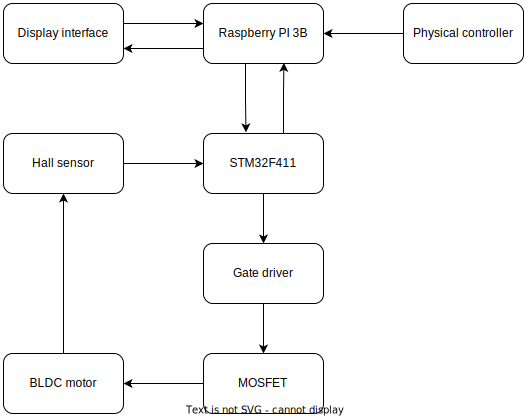
\includegraphics[width=0.3\textwidth]{img/DrawIO/Componentdiagram.svg}
    \caption{Wiring Diagram with Pull-up Resistors}
    \label{fig:hall_sensor_wiring_diagram}
\end{figure}
\section{Sinus}

\subsection{main.c}
\begin{lstlisting}[caption={Activate necessary timers},label={lst:Registers}]
  	HAL_TIM_OC_Start(&htim9, TIM_CHANNEL_1);
  	HAL_TIM_OC_Start(&htim10, TIM_CHANNEL_1);
  	HAL_TIM_PWM_Start(&htim3, TIM_CHANNEL_1);
  	HAL_TIM_PWM_Start(&htim3, TIM_CHANNEL_2);
  	HAL_TIM_PWM_Start(&htim3, TIM_CHANNEL_3);
\end{lstlisting}

\begin{lstlisting}[caption={Start Interrupts},label={lst:Registers}]
  	HAL_TIM_Base_Start_IT(&htim9);
  	HAL_TIM_Base_Start_IT(&htim10);
\end{lstlisting}

\begin{lstlisting}[caption={Fill sintab array},label={lst:Registers}]
	for (int i = 0; i < AANTAL_TIJDSTAPPEN; i++) {
		sintab[i] = sin(i*2*M_PI/AANTAL_TIJDSTAPPEN) * 0.5 + 0.5;
	}
\end{lstlisting}

\begin{lstlisting}[caption={Enable Gate Drivers},label={lst:Registers}]
	GPIOC->ODR = 0xE000;
\end{lstlisting}

\begin{lstlisting}[caption={Read Potentiometer data from ADC for RPM control},label={lst:Registers}]
	HAL_ADC_Start(&hadc1);
	HAL_ADC_PollForConversion(&hadc1, HAL_MAX_DELAY);
	WantedRPM = HAL_ADC_GetValue(&hadc1);
\end{lstlisting}

\begin{lstlisting}[caption={Keep RPM to the minimum set in main.h},label={lst:Registers}]
	if (WantedRPM < MinimumRPM) {
		WantedRPM = MinimumRPM;
	}
\end{lstlisting}

\begin{lstlisting}[caption={Set PSC to appropriate value for RPM},label={lst:Registers}]
	TIM10->PSC = (15 * Fapb2clk) / (256 * WantedRPM) - 1;
\end{lstlisting}

\begin{lstlisting}[caption={Send RPM data to PC},label={lst:Registers}]
	len = snprintf(buf, sizeof(buf), "\n\rWanted RPM / Current RPM: %lu / %lu", WantedRPM, CurrentRPM);
	CDC_Transmit_FS((uint8_t *) buf, len);
	HAL_Delay(10);
\end{lstlisting}

\begin{lstlisting}[caption={i2c instance},label={lst:Registers}]
 hi2c2.Instance = I2C2;
  hi2c2.Init.ClockSpeed = 100000;
  hi2c2.Init.DutyCycle = I2C_DUTYCYCLE_2;
  hi2c2.Init.OwnAddress1 = 0;
  hi2c2.Init.AddressingMode = I2C_ADDRESSINGMODE_7BIT;
  hi2c2.Init.DualAddressMode = I2C_DUALADDRESS_DISABLE;
  hi2c2.Init.OwnAddress2 = 0;
  hi2c2.Init.GeneralCallMode = I2C_GENERALCALL_DISABLE;
  hi2c2.Init.NoStretchMode = I2C_NOSTRETCH_DISABLE;
  if (HAL_I2C_Init(&hi2c2) != HAL_OK)
  {
    Error_Handler();
  }
\end{lstlisting}

\begin{lstlisting}[caption={SPI instance},label={lst:Registers}]
  hspi1.Instance = SPI1;
  hspi1.Init.Mode = SPI_MODE_MASTER;
  hspi1.Init.Direction = SPI_DIRECTION_2LINES;
  hspi1.Init.DataSize = SPI_DATASIZE_8BIT;
  hspi1.Init.CLKPolarity = SPI_POLARITY_LOW;
  hspi1.Init.CLKPhase = SPI_PHASE_1EDGE;
  hspi1.Init.NSS = SPI_NSS_SOFT;
  hspi1.Init.BaudRatePrescaler = SPI_BAUDRATEPRESCALER_2;
  hspi1.Init.FirstBit = SPI_FIRSTBIT_MSB;
  hspi1.Init.TIMode = SPI_TIMODE_DISABLE;
  hspi1.Init.CRCCalculation = SPI_CRCCALCULATION_DISABLE;
  hspi1.Init.CRCPolynomial = 10;
  if (HAL_SPI_Init(&hspi1) != HAL_OK)
  {
    Error_Handler();
  }
\end{lstlisting}

\begin{lstlisting}[caption={TIM3 setup},label={lst:Registers}]
 /* USER CODE END TIM3_Init 1 */
  htim3.Instance = TIM3;
  htim3.Init.Prescaler = 0;
  htim3.Init.CounterMode = TIM_COUNTERMODE_UP;
  htim3.Init.Period = 1919;
  htim3.Init.ClockDivision = TIM_CLOCKDIVISION_DIV1;
  htim3.Init.AutoReloadPreload = TIM_AUTORELOAD_PRELOAD_DISABLE;
  if (HAL_TIM_PWM_Init(&htim3) != HAL_OK)
  {
    Error_Handler();
  }
  sMasterConfig.MasterOutputTrigger = TIM_TRGO_RESET;
  sMasterConfig.MasterSlaveMode = TIM_MASTERSLAVEMODE_DISABLE;
  if (HAL_TIMEx_MasterConfigSynchronization(&htim3, &sMasterConfig) != HAL_OK)
  {
    Error_Handler();
  }
  sConfigOC.OCMode = TIM_OCMODE_PWM1;
  sConfigOC.Pulse = 0;
  sConfigOC.OCPolarity = TIM_OCPOLARITY_HIGH;
  sConfigOC.OCFastMode = TIM_OCFAST_DISABLE;
  if (HAL_TIM_PWM_ConfigChannel(&htim3, &sConfigOC, TIM_CHANNEL_1) != HAL_OK)
  {
    Error_Handler();
  }
  if (HAL_TIM_PWM_ConfigChannel(&htim3, &sConfigOC, TIM_CHANNEL_2) != HAL_OK)
  {
    Error_Handler();
  }
  if (HAL_TIM_PWM_ConfigChannel(&htim3, &sConfigOC, TIM_CHANNEL_3) != HAL_OK)
  {
    Error_Handler();
  }
  /* USER CODE BEGIN TIM3_Init 2 */

  /* USER CODE END TIM3_Init 2 */
  HAL_TIM_MspPostInit(&htim3);

}
\end{lstlisting}

\begin{lstlisting}[caption={Calculate RPM and reset counter},label={lst:Registers}]
	CurrentRPM = 600 * (RPM / 6.0f);
	RPM = 0;
\end{lstlisting}

\begin{lstlisting}[caption={Disable Gate Drivers if RPM is too high},label={lst:Registers}]
	if (CurrentRPM > MaximumRPM) {
		GPIOC->ODR &= 0x1FFF;
	}
\end{lstlisting}

\begin{lstlisting}[caption={Write some registers},label={lst:Registers}]
// Set PWM timers to next step in sinusoid generation
	TIM3->CCR1 = TIM3ARR * sintab[ (j + OffsetU) % AANTAL_TIJDSTAPPEN];
	TIM3->CCR2 = TIM3ARR * sintab[ (j + OffsetV) % AANTAL_TIJDSTAPPEN];
	TIM3->CCR3 = TIM3ARR * sintab[ (j + OffsetW) % AANTAL_TIJDSTAPPEN];

	j++;
\end{lstlisting}

\begin{lstlisting}[caption={Write some registers},label={lst:Registers}]
	if( j > AANTAL_TIJDSTAPPEN) {
		j = 0; // Reset j when full sinusoid has been made.
	}
\end{lstlisting}

\section{Commutation}
\subsection{main.c}
\begin{lstlisting}[caption={Write some registers},label={lst:Registers}]
uint8_t HallSensor = 0;
uint16_t Commutation[6][3] = {
		{0x0, 0xF, 0xF},
		{},
		{},
		{},
		{},
		{}
};
\end{lstlisting}

\begin{lstlisting}[caption={Write some registers},label={lst:Registers}]
HAL_StatusTypeDef StartupSequence(char Direction);
HAL_StatusTypeDef PrepareCommutation(void);
\end{lstlisting}

\begin{lstlisting}[caption={Write some registers},label={lst:Registers}]
  TIM1->CR2 |= 0x0005; 			// Set CCPC 1 and CCUS 1 in CR2
  TIM1->SR &= ~TIM_SR_COMIF; 	// Set COMIF low in SR to not trigger commutation event
  TIM1->DIER |= TIM_DIER_COMIE; // Enable Commutation events in DIER register

  StartupSequence('F');
\end{lstlisting}

\begin{lstlisting}[caption={Set first commutation state according to Hall sensors},label={lst:Registers}]
HAL_StatusTypeDef StartupSequence(char Direction) {

  if (PrepareCommutation() == HAL_ERROR) {
	  return HAL_ERROR;
  }

  // Start HallSensor timer
  HAL_TIMEx_HallSensor_Start(&htim2);

  // Start all PWM signals on TIM1
  HAL_TIM_PWM_Start(&htim1, TIM_CHANNEL_1);
  HAL_TIM_PWM_Start(&htim1, TIM_CHANNEL_2);
  HAL_TIM_PWM_Start(&htim1, TIM_CHANNEL_3);

  // Start Interrupts
  HAL_TIM_Base_Start_IT(&htim2);
  HAL_TIM_Base_Start_IT(&htim1);

  // Set COMG bit in EGR for first commutation
  TIM1->EGR |= TIM_EGR_COMG;

  return HAL_OK;

}

HAL_StatusTypeDef PrepareCommutation() {

  // Read IDR for Hall Sensor status
  uint8_t Hall = GPOIA->IDR & 0x0007;

  switch (Hall) {
  case 0b001:
	  HallSensor = 0;
  break;
  }

  return HAL_OK;

}
\end{lstlisting}



\subsection{stm32f4xx\textunderscore it.c}
\begin{lstlisting}[caption={Set new Commutation states CCxE, CCxNE, OCxM in CCER and CCMR1 and CCMR2 according to array},label={lst:Registers}]
void TIM1_TRG_COM_TIM11_IRQHandler(void)
{
  /* USER CODE BEGIN TIM1_TRG_COM_TIM11_IRQn 0 */

	// Set new Commutation states CCxE, CCxNE, OCxM in CCER and CCMR1 and CCMR2 according to array
	// Reset COMIF in SR register


  /* USER CODE END TIM1_TRG_COM_TIM11_IRQn 0 */
  HAL_TIM_IRQHandler(&htim1);
  /* USER CODE BEGIN TIM1_TRG_COM_TIM11_IRQn 1 */

  /* USER CODE END TIM1_TRG_COM_TIM11_IRQn 1 */
}

/**
  * @brief This function handles TIM2 global interrupt.
  */
void TIM2_IRQHandler(void)
{
  /* USER CODE BEGIN TIM2_IRQn 0 */

  // Set COMG bit in EGR
  TIM1->EGR |= TIM_EGR_COMG;

  /* USER CODE END TIM2_IRQn 0 */
  HAL_TIM_IRQHandler(&htim2);
  /* USER CODE BEGIN TIM2_IRQn 1 */

  /* USER CODE END TIM2_IRQn 1 */
}
\end{lstlisting}

% \section{Sinus}

\subsection{main.c}
\begin{lstlisting}[caption={Activate necessary timers},label={lst:Registers}]
  	HAL_TIM_OC_Start(&htim9, TIM_CHANNEL_1);
  	HAL_TIM_OC_Start(&htim10, TIM_CHANNEL_1);
  	HAL_TIM_PWM_Start(&htim3, TIM_CHANNEL_1);
  	HAL_TIM_PWM_Start(&htim3, TIM_CHANNEL_2);
  	HAL_TIM_PWM_Start(&htim3, TIM_CHANNEL_3);
\end{lstlisting}

\begin{lstlisting}[caption={Start Interrupts},label={lst:Registers}]
  	HAL_TIM_Base_Start_IT(&htim9);
  	HAL_TIM_Base_Start_IT(&htim10);
\end{lstlisting}

\begin{lstlisting}[caption={Fill sintab array},label={lst:Registers}]
	for (int i = 0; i < AANTAL_TIJDSTAPPEN; i++) {
		sintab[i] = sin(i*2*M_PI/AANTAL_TIJDSTAPPEN) * 0.5 + 0.5;
	}
\end{lstlisting}

\begin{lstlisting}[caption={Enable Gate Drivers},label={lst:Registers}]
	GPIOC->ODR = 0xE000;
\end{lstlisting}

\begin{lstlisting}[caption={Read Potentiometer data from ADC for RPM control},label={lst:Registers}]
	HAL_ADC_Start(&hadc1);
	HAL_ADC_PollForConversion(&hadc1, HAL_MAX_DELAY);
	WantedRPM = HAL_ADC_GetValue(&hadc1);
\end{lstlisting}

\begin{lstlisting}[caption={Keep RPM to the minimum set in main.h},label={lst:Registers}]
	if (WantedRPM < MinimumRPM) {
		WantedRPM = MinimumRPM;
	}
\end{lstlisting}

\begin{lstlisting}[caption={Set PSC to appropriate value for RPM},label={lst:Registers}]
	TIM10->PSC = (15 * Fapb2clk) / (256 * WantedRPM) - 1;
\end{lstlisting}

\begin{lstlisting}[caption={Send RPM data to PC},label={lst:Registers}]
	len = snprintf(buf, sizeof(buf), "\n\rWanted RPM / Current RPM: %lu / %lu", WantedRPM, CurrentRPM);
	CDC_Transmit_FS((uint8_t *) buf, len);
	HAL_Delay(10);
\end{lstlisting}

\begin{lstlisting}[caption={i2c instance},label={lst:Registers}]
 hi2c2.Instance = I2C2;
  hi2c2.Init.ClockSpeed = 100000;
  hi2c2.Init.DutyCycle = I2C_DUTYCYCLE_2;
  hi2c2.Init.OwnAddress1 = 0;
  hi2c2.Init.AddressingMode = I2C_ADDRESSINGMODE_7BIT;
  hi2c2.Init.DualAddressMode = I2C_DUALADDRESS_DISABLE;
  hi2c2.Init.OwnAddress2 = 0;
  hi2c2.Init.GeneralCallMode = I2C_GENERALCALL_DISABLE;
  hi2c2.Init.NoStretchMode = I2C_NOSTRETCH_DISABLE;
  if (HAL_I2C_Init(&hi2c2) != HAL_OK)
  {
    Error_Handler();
  }
\end{lstlisting}

\begin{lstlisting}[caption={SPI instance},label={lst:Registers}]
  hspi1.Instance = SPI1;
  hspi1.Init.Mode = SPI_MODE_MASTER;
  hspi1.Init.Direction = SPI_DIRECTION_2LINES;
  hspi1.Init.DataSize = SPI_DATASIZE_8BIT;
  hspi1.Init.CLKPolarity = SPI_POLARITY_LOW;
  hspi1.Init.CLKPhase = SPI_PHASE_1EDGE;
  hspi1.Init.NSS = SPI_NSS_SOFT;
  hspi1.Init.BaudRatePrescaler = SPI_BAUDRATEPRESCALER_2;
  hspi1.Init.FirstBit = SPI_FIRSTBIT_MSB;
  hspi1.Init.TIMode = SPI_TIMODE_DISABLE;
  hspi1.Init.CRCCalculation = SPI_CRCCALCULATION_DISABLE;
  hspi1.Init.CRCPolynomial = 10;
  if (HAL_SPI_Init(&hspi1) != HAL_OK)
  {
    Error_Handler();
  }
\end{lstlisting}

\begin{lstlisting}[caption={TIM3 setup},label={lst:Registers}]
 /* USER CODE END TIM3_Init 1 */
  htim3.Instance = TIM3;
  htim3.Init.Prescaler = 0;
  htim3.Init.CounterMode = TIM_COUNTERMODE_UP;
  htim3.Init.Period = 1919;
  htim3.Init.ClockDivision = TIM_CLOCKDIVISION_DIV1;
  htim3.Init.AutoReloadPreload = TIM_AUTORELOAD_PRELOAD_DISABLE;
  if (HAL_TIM_PWM_Init(&htim3) != HAL_OK)
  {
    Error_Handler();
  }
  sMasterConfig.MasterOutputTrigger = TIM_TRGO_RESET;
  sMasterConfig.MasterSlaveMode = TIM_MASTERSLAVEMODE_DISABLE;
  if (HAL_TIMEx_MasterConfigSynchronization(&htim3, &sMasterConfig) != HAL_OK)
  {
    Error_Handler();
  }
  sConfigOC.OCMode = TIM_OCMODE_PWM1;
  sConfigOC.Pulse = 0;
  sConfigOC.OCPolarity = TIM_OCPOLARITY_HIGH;
  sConfigOC.OCFastMode = TIM_OCFAST_DISABLE;
  if (HAL_TIM_PWM_ConfigChannel(&htim3, &sConfigOC, TIM_CHANNEL_1) != HAL_OK)
  {
    Error_Handler();
  }
  if (HAL_TIM_PWM_ConfigChannel(&htim3, &sConfigOC, TIM_CHANNEL_2) != HAL_OK)
  {
    Error_Handler();
  }
  if (HAL_TIM_PWM_ConfigChannel(&htim3, &sConfigOC, TIM_CHANNEL_3) != HAL_OK)
  {
    Error_Handler();
  }
  /* USER CODE BEGIN TIM3_Init 2 */

  /* USER CODE END TIM3_Init 2 */
  HAL_TIM_MspPostInit(&htim3);

}
\end{lstlisting}

\begin{lstlisting}[caption={Calculate RPM and reset counter},label={lst:Registers}]
	CurrentRPM = 600 * (RPM / 6.0f);
	RPM = 0;
\end{lstlisting}

\begin{lstlisting}[caption={Disable Gate Drivers if RPM is too high},label={lst:Registers}]
	if (CurrentRPM > MaximumRPM) {
		GPIOC->ODR &= 0x1FFF;
	}
\end{lstlisting}

\begin{lstlisting}[caption={Write some registers},label={lst:Registers}]
// Set PWM timers to next step in sinusoid generation
	TIM3->CCR1 = TIM3ARR * sintab[ (j + OffsetU) % AANTAL_TIJDSTAPPEN];
	TIM3->CCR2 = TIM3ARR * sintab[ (j + OffsetV) % AANTAL_TIJDSTAPPEN];
	TIM3->CCR3 = TIM3ARR * sintab[ (j + OffsetW) % AANTAL_TIJDSTAPPEN];

	j++;
\end{lstlisting}

\begin{lstlisting}[caption={Write some registers},label={lst:Registers}]
	if( j > AANTAL_TIJDSTAPPEN) {
		j = 0; // Reset j when full sinusoid has been made.
	}
\end{lstlisting}

\section{Commutation}
\subsection{main.c}
\begin{lstlisting}[caption={Write some registers},label={lst:Registers}]
uint8_t HallSensor = 0;
uint16_t Commutation[6][3] = {
		{0x0, 0xF, 0xF},
		{},
		{},
		{},
		{},
		{}
};
\end{lstlisting}

\begin{lstlisting}[caption={Write some registers},label={lst:Registers}]
HAL_StatusTypeDef StartupSequence(char Direction);
HAL_StatusTypeDef PrepareCommutation(void);
\end{lstlisting}

\begin{lstlisting}[caption={Write some registers},label={lst:Registers}]
  TIM1->CR2 |= 0x0005; 			// Set CCPC 1 and CCUS 1 in CR2
  TIM1->SR &= ~TIM_SR_COMIF; 	// Set COMIF low in SR to not trigger commutation event
  TIM1->DIER |= TIM_DIER_COMIE; // Enable Commutation events in DIER register

  StartupSequence('F');
\end{lstlisting}

\begin{lstlisting}[caption={Set first commutation state according to Hall sensors},label={lst:Registers}]
HAL_StatusTypeDef StartupSequence(char Direction) {

  if (PrepareCommutation() == HAL_ERROR) {
	  return HAL_ERROR;
  }

  // Start HallSensor timer
  HAL_TIMEx_HallSensor_Start(&htim2);

  // Start all PWM signals on TIM1
  HAL_TIM_PWM_Start(&htim1, TIM_CHANNEL_1);
  HAL_TIM_PWM_Start(&htim1, TIM_CHANNEL_2);
  HAL_TIM_PWM_Start(&htim1, TIM_CHANNEL_3);

  // Start Interrupts
  HAL_TIM_Base_Start_IT(&htim2);
  HAL_TIM_Base_Start_IT(&htim1);

  // Set COMG bit in EGR for first commutation
  TIM1->EGR |= TIM_EGR_COMG;

  return HAL_OK;

}

HAL_StatusTypeDef PrepareCommutation() {

  // Read IDR for Hall Sensor status
  uint8_t Hall = GPOIA->IDR & 0x0007;

  switch (Hall) {
  case 0b001:
	  HallSensor = 0;
  break;
  }

  return HAL_OK;

}
\end{lstlisting}



\subsection{stm32f4xx\textunderscore it.c}
\begin{lstlisting}[caption={Set new Commutation states CCxE, CCxNE, OCxM in CCER and CCMR1 and CCMR2 according to array},label={lst:Registers}]
void TIM1_TRG_COM_TIM11_IRQHandler(void)
{
  /* USER CODE BEGIN TIM1_TRG_COM_TIM11_IRQn 0 */

	// Set new Commutation states CCxE, CCxNE, OCxM in CCER and CCMR1 and CCMR2 according to array
	// Reset COMIF in SR register


  /* USER CODE END TIM1_TRG_COM_TIM11_IRQn 0 */
  HAL_TIM_IRQHandler(&htim1);
  /* USER CODE BEGIN TIM1_TRG_COM_TIM11_IRQn 1 */

  /* USER CODE END TIM1_TRG_COM_TIM11_IRQn 1 */
}

/**
  * @brief This function handles TIM2 global interrupt.
  */
void TIM2_IRQHandler(void)
{
  /* USER CODE BEGIN TIM2_IRQn 0 */

  // Set COMG bit in EGR
  TIM1->EGR |= TIM_EGR_COMG;

  /* USER CODE END TIM2_IRQn 0 */
  HAL_TIM_IRQHandler(&htim2);
  /* USER CODE BEGIN TIM2_IRQn 1 */

  /* USER CODE END TIM2_IRQn 1 */
}
\end{lstlisting}

% \include{information/appendix} %% DEZE VERWIJDEREN MITS DIE FILE NIET MEER NODIG IS
\nocite{*}
\include{information/Sources}

\appendix
% \input{appendix/python/Pythonopmaak}
% \input{appendix/python/complex.py}
% \input{appendix/stm32_specs}
% \input{appendix/C/halsensor.c}
\end{document}
